%=======================================================================
% SAHAi — Preliminary Technical Report (IEEE conference format)
%
% Compile:  pdflatex sahai_preliminary_report.tex   (twice, for refs)
% Needs:    IEEEtran, pgfplots, booktabs, amsmath
% Figure:   figures/architecture.png must sit beside this file.
%
% REFERENCES: titles for [1]-[3] are taken verbatim from the project's own
% literature review. Author lists, venues and years are not recorded there
% and are marked "% FILL IN". Nothing here was invented.
%=======================================================================
\documentclass[conference]{IEEEtran}
\IEEEoverridecommandlockouts

\usepackage{cite}
\usepackage{amsmath,amssymb,amsfonts}
\usepackage{algorithmic}
\usepackage{graphicx}
\usepackage{textcomp}
\usepackage{xcolor}
\usepackage{booktabs}
\usepackage{array}
\usepackage{url}
\usepackage{balance}
\usepackage{microtype}
\usepackage{enumitem}
\usepackage{tabularx}
\usepackage{pgfplots}
\pgfplotsset{compat=1.17}
\usepackage[hidelinks]{hyperref}

\def\BibTeX{{\rm B\kern-.05em{\sc i\kern-.025em b}\kern-.08em
    T\kern-.1667em\lower.7ex\hbox{E}\kern-.125emX}}

%-----------------------------------------------------------------------
% The supplied preamble also set geometry/setspace/parskip. They are kept
% here but disabled: each overrides IEEEtran and the output would no
% longer be IEEE conference format. Uncomment only if a rubric demands it.
%
% \usepackage{geometry}\usepackage{setspace}\usepackage{parskip}
% \geometry{left=25mm,right=25mm,top=25mm,bottom=25mm}
% \setlength{\parindent}{0pt}\onehalfspacing
%-----------------------------------------------------------------------

\begin{document}

\title{SAHAi: Reinforcement Learning of a Non-Answer-Giving\\Programming Tutor Against a Simulated Student}

\author{
    \IEEEauthorblockN{
        Aishwarya Manoj\textsuperscript{1},
        Aswathi Ranjith\textsuperscript{1},
        Harshita Chandrashekar\textsuperscript{1},
        Lakshmi Ridhanya\textsuperscript{1}
    }
    \IEEEauthorblockA{
        Amrita School of Artificial Intelligence \\
        Amrita Vishwa Vidyapeetham, Coimbatore, India \\
        Emails: \{cb.sc.u4aie23211, cb.sc.u4aie23215, cb.sc.u4aie23231, cb.sc.u4aie23270\}@cb.students.amrita.edu \\
        \textsuperscript{1}First Authors
    }
}

\maketitle

\begin{abstract}
Competence at solving a programming problem does not confer competence at
teaching one, and the two pull against each other: the fastest route to a
correct submission is to disclose the answer. We describe SAHAi, which trains a small
(1.5B-parameter) tutor policy by critic-free reinforcement learning against
a simulated student, using no corpus of human tutoring dialogue.
Supervision comes from the student's execution-verified downstream success,
penalised for solution leakage and for non-pedagogical behaviour, with an
explicit Bayesian learner model supplying the ability baseline and driving
curriculum selection. We also describe the deployed interactive system
built around the trained policy. Our central result is negative and
stated as such: the best held-out solve rate, $17.5\%$ over 20 unseen
problems, is the highest recorded across seven runs but is statistically
indistinguishable from the previous best of $16.3\%$ at the dispersion the
evaluation set permits. We explain why, and the explanation is the paper's
main contribution. Whatever the tutor can score from its own output dominates the usable
gradient by roughly five to one over the outcome the system exists to
optimise, so the estimator trains the former and reads the latter as noise.
A second result is sharper: scoring pedagogy as a conjunction of judge
verdicts, which is how the source specification defines it, collapses the
advantage estimate to zero and halts learning outright. Both findings
transfer to any system porting a reward designed for PPO onto a criticless
algorithm.
\end{abstract}

\begin{IEEEkeywords}
reinforcement learning from verifiable rewards, group-relative policy
optimization, intelligent tutoring systems, simulated learners, knowledge
tracing, reward hacking, large language models
\end{IEEEkeywords}

%=======================================================================
\section{Introduction}
%=======================================================================

A language model that can solve a programming problem is not, by
construction, a model that can \emph{teach} it. The two behaviours are in
direct tension: the fastest way to make a learner's next submission correct
is to hand them the answer, which is precisely what tutoring exists to
avoid.

SAHAi treats this as a reinforcement learning problem. A tutor policy
$\pi_\theta$ holds a multi-turn dialogue with a \emph{simulated} student;
the student then attempts the problem; the attempt is executed against unit
tests; and the tutor is rewarded for the student's verified success while
being penalised for disclosing the solution. No corpus of human tutoring
dialogues is used anywhere. This follows the source
review~\cite{rev-pedrl}, which objects to supervised fine-tuning on
teacher--student transcripts on the grounds that few high-quality tutoring
corpora exist publicly.

This report is preliminary, and we state its limits at the outset. Seven
training runs have completed. Held-out solve rate has never left the
$6$--$18\%$ band, and no run-to-run difference in that band is resolvable
at the evaluation set size used. Two things are established. The first is a set of reproducible results
about how reward design behaves under a criticless estimator, each tied to
a measurement rather than to an opinion. The second is a working
interactive system built around the policy.

\subsection{Contributions}
\begin{enumerate}[leftmargin=*,topsep=2pt]
\item A working, execution-grounded training pipeline for pedagogical RL
      against a simulated learner (Sec.~\ref{sec:method}), and a deployed
      interactive system in which the same pedagogy and leakage
      definitions that are optimised are also the ones served
      (Sec.~\ref{sec:interactive}).
\item A structural incompatibility result: a conversation-level
      \emph{binary} pedagogy reward, as specified for actor--critic
      optimisation, yields exactly zero gradient under group-relative
      advantage estimation (Sec.~\ref{sec:binary}).
\item A quantified reward-channel asymmetry: the terms that are
      deterministic functions of the tutor's own text carry roughly five
      times the within-group variance of the outcome term the system
      exists to optimise, which explains why six successive corrections
      did not move generalisation (Sec.~\ref{sec:channel}).
\item A statistical-power result on our own protocol: the held-out set
      used for every run-to-run comparison to date cannot resolve the
      differences it was used to judge (Sec.~\ref{sec:threats}).
\end{enumerate}

%=======================================================================
\section{Method}
\label{sec:method}
%=======================================================================

\begin{figure*}[!t]
\centering
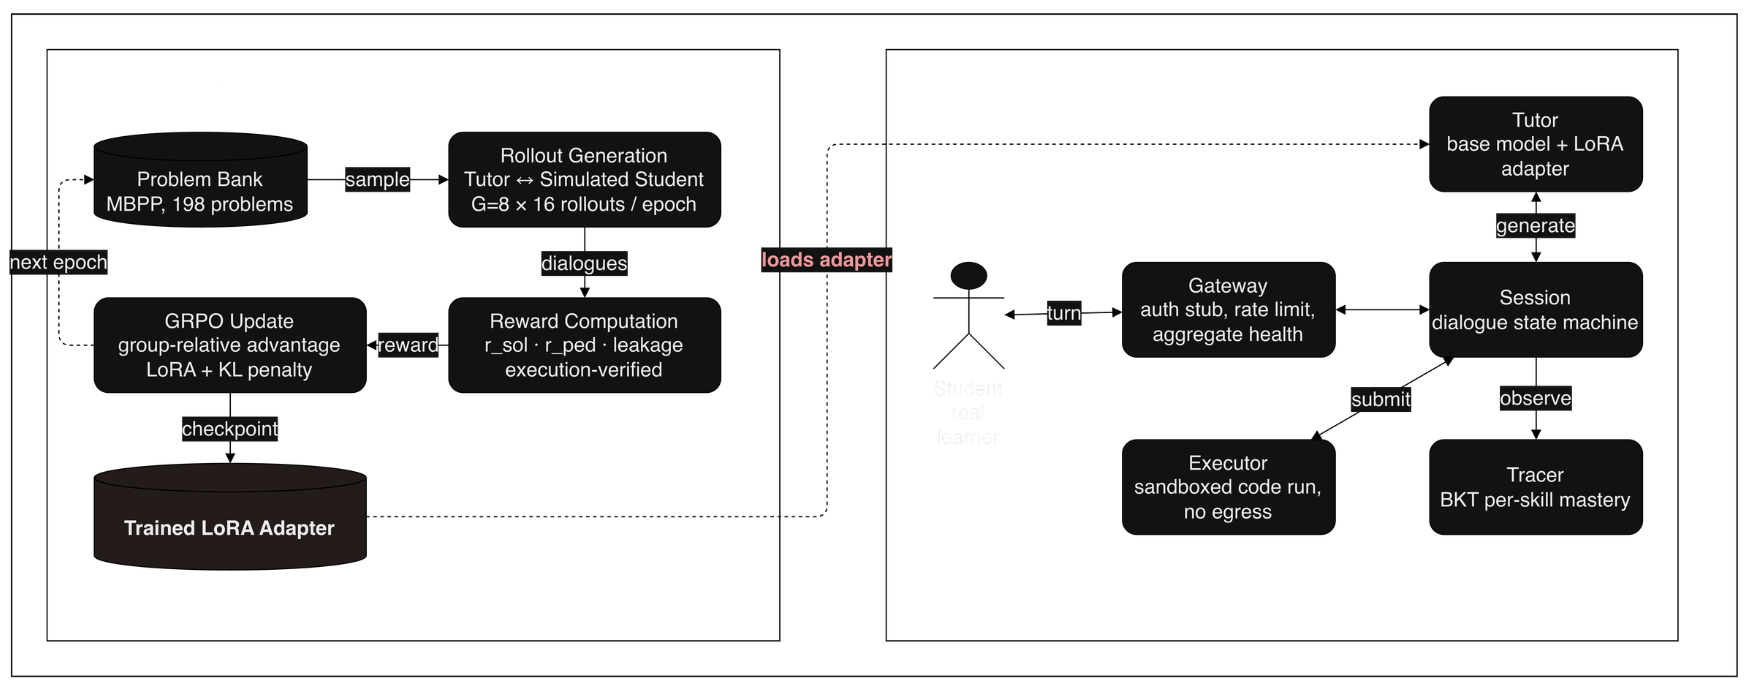
\includegraphics[width=\textwidth]{figures/architecture.png}
\caption{The two halves of SAHAi and the single artifact joining them.
\textbf{Left (training):} problems are drawn from the bank by the
curriculum sampler; the tutor policy and simulated student generate a group
of dialogues per problem; each completed dialogue is scored by the
execution-verified reward of \eqref{eq:reward}; the group-relative update
writes a low-rank adapter. \textbf{Right (serving):} a real learner reaches
the gateway, the session service orchestrates the turn against the tutor,
submitted code runs in the no-egress executor, and the tracer updates
per-skill mastery. The adapter produced on the left is the only thing that
crosses to the right. The reported run used 4 problems per epoch with
$G{=}8$, i.e.\ 32 rollouts per epoch; see Table~\ref{tab:config}.}
\label{fig:arch}
\end{figure*}

\subsection{Group-relative optimisation}

Policy-gradient methods optimise
$J(\theta)=\mathbb{E}_{\tau\sim\pi_\theta}[R(\tau)]$. PPO~\cite{ppo}
stabilises this with a clipped importance ratio against a learned value
baseline. Group Relative Policy Optimization~\cite{grpo} removes the value
network: for a group of $G$ trajectories sampled on the same prompt, the
advantage of trajectory $i$ is the within-group $z$-score
\begin{equation}
A_i=\frac{r_i-\mu_{\text{group}}}{\sigma_{\text{group}}+\epsilon}.
\label{eq:adv}
\end{equation}
This halves optimiser memory and removes value-function tuning, at a cost
central to this report: \textbf{within-group reward variance is the entire
learning signal}. A group whose members score identically contributes zero
gradient, a property PPO's learned baseline does not share. Without the
importance ratio, \eqref{eq:adv} reduces to REINFORCE~\cite{reinforce} with
a $z$-scored baseline.

\subsection{Rollout and the simulated student}

For each sampled problem, $G$ dialogues are generated (Fig.~\ref{fig:arch}).
The student opens with a scripted in-persona utterance; tutor and student
then alternate until a termination phrase or a turn cap. Only tokens
emitted by the tutor enter the loss, via an assistant-span mask; this is
why the student's output may be post-processed and the tutor's may not.

The student is a frozen, 4-bit-quantised instruction model~\cite{qwen}
carrying a persona~\cite{rev-simstudents}: an ability level, per-skill
misconceptions injected into its prompt, and a code-mixing register
(Hinglish, Tanglish or English). It is paired with a Bayesian Knowledge
Tracing~\cite{bkt} model maintaining a per-skill mastery posterior, updated
after every rollout. Ability is obtained from the tracer, never by asking a
model to judge itself~\cite{rev-learnermodel}. Deep Knowledge
Tracing~\cite{dkt} was rejected on data scale: it requires interaction logs
a synthetic student does not produce, whereas BKT is usable from a single
observation and yields a named-skill value that both the ability baseline
and the curriculum sampler require.

\subsection{Reward}

The conversation-level reward is
\begin{equation}
r_{\mathrm{SAHAI}}=\bigl(r_{\mathrm{sol}}-\alpha\bigr)
+\bigl(r_{\mathrm{ped}}-1\bigr)\lambda-\gamma L,
\label{eq:reward}
\end{equation}
with a hard penalty $r_{\mathrm{SAHAI}}=-\lambda$ when
$r_{\mathrm{ped}}=0$. The terms are:
\begin{itemize}[leftmargin=*,topsep=2pt,itemsep=1pt,parsep=0pt]
\item $r_{\mathrm{sol}}$, the post-dialogue solve rate, obtained by
      executing the student's attempt in a sandbox against the problem's
      unit tests.
\item $\alpha$, the tracer's ability baseline. Subtracting it denies
      the tutor credit for a student who could already solve the problem.
\item $r_{\mathrm{ped}}$, a graded rule-based judge averaging three
      checks, all of the form ``did the tutor give the answer away''.
\item $L\in[0,1]$, the leakage term. It combines rare-token overlap
      between tutor text and the reference solution, with
      problem-statement tokens subtracted, plus an execution check under
      which tutor-written code that passes the problem's own tests scores
      $L{=}1$ regardless of lexical similarity.
\end{itemize}

Advantages follow \eqref{eq:adv} over groups sharing a problem. The loss
adds a KL penalty to a frozen reference policy, realised as the same
weights with adapters disabled. Problems are drawn by a curriculum sampler
operating on the tracer's mastery state, following the Zone of Proximal
Development~\cite{vygotsky}.

%=======================================================================
\section{The Interactive System}
\label{sec:interactive}
%=======================================================================

A trained adapter is not a usable tutor. The serving half of SAHAi is a
six-service containerised stack. It is described here for two reasons: two
of its constraints fed back into the training design, as the next two
paragraphs set out, and it is the part of the project that is finished,
which the training half is not.

\textbf{The boundary.} The research prototype conflated two situations that
behave differently. In training, the student is a model driven in a loop,
control flow is batch, and mastery state is synthetic and discarded. In
production, the student is a person sending one turn and waiting, state
must survive restarts, and mastery belongs to that person permanently. The
dialogue engine therefore became two things, a batch runner for RL and a
state machine over a persisted transcript. Both score through one shared
domain library, so that pedagogy and leakage cannot drift apart
between what is optimised and what is served.

\textbf{Containment.} The security-relevant property is that \emph{scoring}
is separated from \emph{execution}. In the prototype, the code verifier
sat beside the reward logic, so anything importing the reward stack
inherited the ability to execute arbitrary model output. In the deployed
system the shared library is enforced by test to expose no code runner at
all, and untrusted code runs only in an executor container whose
containment is layered: an internal-only network with no egress, a
read-only root filesystem, a non-root user with all capabilities dropped,
process and memory limits, and a fresh interpreter per test case. The
verdict is read from a sentinel line, so a candidate program's own output
can neither corrupt nor forge it.

\textbf{Learner interface.} Three pages are served: a workspace with a
problem picker, the tutoring conversation, a code editor with
submit-and-run, a live per-skill mastery panel and a microphone control; a
progress page showing streak, activity grid, per-skill mastery, course
tracks and a next-problem recommendation; and a timed, graded coding
placement. Two behaviours were failures first. A turn is \emph{atomic}: the
learner's turn was previously committed before the tutor was called, so a
timeout left a turn with no reply and a retry appended a second learner
turn, breaking the role alternation that prompt assembly and the pedagogy
judge both assume, with no error raised anywhere. A response for a
conversation the learner has left is \emph{discarded, not rendered}, using
an epoch token compared on arrival.

\textbf{Voice.} Speech wraps the existing text path rather than
duplicating it: the websocket handler calls the same turn endpoint the text
box calls, and so inherits learner context and problem statement. Stages
are reported as they complete rather than batched, because recognition
takes seconds while generation can take minutes. On the development host,
a CPU-only container runtime, Indic recognition completed in $13$--$34$\,s
and is usable, whereas Indic synthesis did not finish a 16-character
sentence within $840$\,s; synthesis is therefore budgeted and degrades to
text-only. These are single-host observations, not a benchmark.

\textbf{Learner state and turn adaptation.} Priors are seeded either by a
self-assessment, mapped into $[0.15,0.65]$ because a self-report is
evidence rather than proof, or by importing a public repository of solved
problems. In the latter, source is parsed and discarded at the import
boundary: only skill tags and one technique phrase per problem are
retained, never a line of code. Streak, activity, mastery and track
completion are all projected from a single append-only observation log
rather than from separate tables. Finally, a high-precision rule layer
reads what the learner just wrote, in English and romanized Hindi and
Tamil, to tell whether they are stuck, asking to be handed the answer, or
posting an attempt. It is rule-based because the tutor already owns
$200$\,s of a $240$\,s turn budget; a fourth rule, recognising a proposed
approach, is deliberately absent because no cheap detector separates
proposing from guessing, and the design rule is that detection must stay
silent when unsure.

\textbf{Invariants and gaps.} Each hop outlasts the one it calls
($270>240>200$\,s); inverted, the outer caller abandons a request the inner
one was about to answer, and a real turn was lost this way. Every model
call carries its own deadline, since a client timeout does not cancel
server-side work. Identity is a bearer token of which only a hash is
stored, which authenticates a bearer rather than a person, and the internal
hop rests on network topology rather than cryptography.

%=======================================================================
\section{Experimental Setup}
\label{sec:setup}
%=======================================================================

\begin{table}[t]
\caption{Configuration of the reported run}
\label{tab:config}
\centering
\small
\begin{tabular}{ll}
\toprule
\textbf{Component} & \textbf{Setting} \\
\midrule
Tutor policy      & Qwen2.5-1.5B-Instruct + LoRA~\cite{lora} \\
Adapter           & rank 8, $\alpha=16$, $q/k/v/o$ projections \\
Student simulator & Qwen2.5-1.5B-Instruct, 4-bit, frozen \\
Judge             & rule-based, 3 graded checks \\
Problem bank      & MBPP~\cite{mbpp} train split; 198 loaded \\
Held-out set      & 20 unseen problems \\
Epochs            & 10 \\
Batch             & 4 problems $\times$ $G=8$ $=32$ rollouts/epoch \\
Total rollouts    & 320 dialogues \\
Max turns         & 4 \\
Solve samples     & 4 \\
Learning rate     & $1\times10^{-4}$ \\
KL coefficient    & 0.05 \\
Optimiser steps   & 16 per epoch \\
$\lambda$, $\gamma$ & 1.0, 0.5 \\
Hardware          & NVIDIA T4 $\times$ 2 \\
Wall clock        & 32{,}995\,s ($\approx$9.2\,h), completed \\
\bottomrule
\end{tabular}
\end{table}

Table~\ref{tab:config} gives the configuration. A rule-based judge is used
rather than the multiple LLM judges the source review recommends, because a
third model does not fit alongside tutor and student on one 16\,GB
accelerator. The consequence is acknowledged rather than hidden: the
pedagogy term is a heuristic, gameable in ways an LLM judge would not be,
and the judge-holdout protection recommended in the
review~\cite{rev-simstudents} is absent.

After training, the final adapter is run on held-out problems; each yields
one dialogue and one scored student attempt, and the reported solve rate is
the mean over those problems. Leakage at evaluation is fitted on the
\emph{training} corpus, so that ``rare token'' means the same thing in both
phases. All values below are taken from the artifacts of a single completed
run, inspected directly.

%=======================================================================
\section{Results}
\label{sec:results}
%=======================================================================

\begin{table}[t]
\caption{Per-epoch training metrics. \emph{solve} is the mean of
$r_{\mathrm{sol}}$ over the epoch's 32 rollouts.}
\label{tab:epochs}
\centering
\small
\begin{tabular}{rrrrrr}
\toprule
\textbf{Ep} & \textbf{loss} & \textbf{KL} & \textbf{reward} &
\textbf{solve} & \textbf{ped} \\
\midrule
0 & 0.0923 & 0.0003 & $-0.576$ & 0.086 & 0.802 \\
1 & 0.0973 & 0.0021 & $-0.820$ & 0.063 & 0.661 \\
2 & 0.0538 & 0.0069 & $-0.288$ & 0.156 & 0.904 \\
3 & 0.0543 & 0.0096 & $-0.399$ & 0.000 & 0.922 \\
4 & 0.0492 & 0.0096 & $-0.223$ & 0.039 & 0.981 \\
5 & 0.0399 & 0.0139 & $+0.026$ & 0.219 & 0.997 \\
6 & 0.0166 & 0.0231 & $-0.344$ & 0.008 & 0.978 \\
7 & 0.0089 & 0.0301 & $+0.108$ & 0.344 & 0.984 \\
8 & 0.0393 & 0.0242 & $+0.124$ & 0.273 & 0.997 \\
9 & $-0.0420$ & 0.0242 & $+0.071$ & 0.297 & 0.988 \\
\midrule
\multicolumn{2}{l}{$\mathrm{corr}(\text{epoch},\cdot)$}
 & $+0.94$ & $+0.86$ & $+0.65$ & $+0.77$ \\
\bottomrule
\end{tabular}
\end{table}

\begin{figure}[t]
\centering
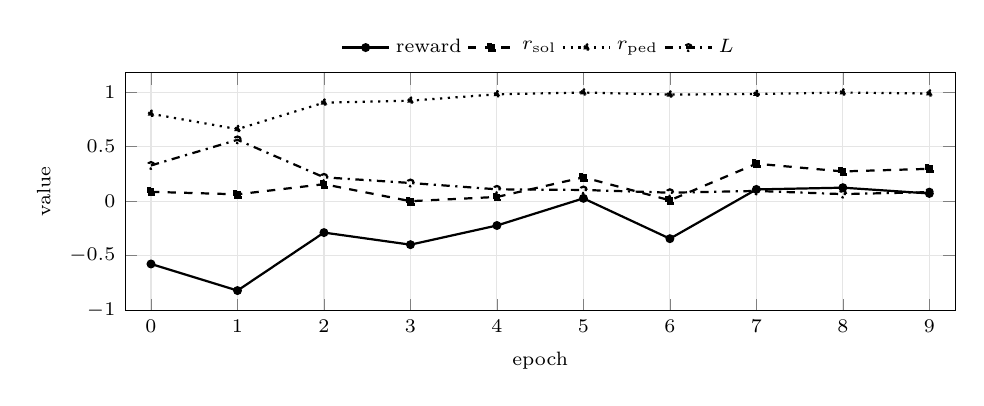
\begin{tikzpicture}
\begin{axis}[
  width=\columnwidth, height=4.6cm,
  xlabel={epoch}, ylabel={value},
  xmin=-0.3, xmax=9.3,
  legend style={font=\scriptsize, at={(0.5,1.02)}, anchor=south,
                legend columns=4, draw=none},
  grid=major, grid style={gray!20},
  tick label style={font=\scriptsize}, label style={font=\scriptsize},
]
\addplot[thick, mark=*, mark size=1.2pt] coordinates {
 (0,-0.576)(1,-0.820)(2,-0.288)(3,-0.399)(4,-0.223)
 (5,0.026)(6,-0.344)(7,0.108)(8,0.124)(9,0.071)};
\addlegendentry{reward}
\addplot[thick, mark=square*, mark size=1.2pt, dashed] coordinates {
 (0,0.086)(1,0.063)(2,0.156)(3,0.000)(4,0.039)
 (5,0.219)(6,0.008)(7,0.344)(8,0.273)(9,0.297)};
\addlegendentry{$r_{\mathrm{sol}}$}
\addplot[thick, mark=triangle*, mark size=1.4pt, dotted] coordinates {
 (0,0.802)(1,0.661)(2,0.904)(3,0.922)(4,0.981)
 (5,0.997)(6,0.978)(7,0.984)(8,0.997)(9,0.988)};
\addlegendentry{$r_{\mathrm{ped}}$}
\addplot[thick, mark=o, mark size=1.2pt, dashdotted] coordinates {
 (0,0.328)(1,0.563)(2,0.219)(3,0.167)(4,0.109)
 (5,0.103)(6,0.078)(7,0.094)(8,0.065)(9,0.083)};
\addlegendentry{$L$}
\end{axis}
\end{tikzpicture}
\caption{Training-epoch reward components. The deterministic,
tutor-controlled terms ($r_{\mathrm{ped}}$, $L$) move smoothly in the
intended direction; the outcome term $r_{\mathrm{sol}}$ oscillates with an
epoch-to-epoch standard deviation of $0.121$, roughly $3.8\times$ the
$0.031$ expected from sampling alone.}
\label{fig:curves}
\end{figure}

\subsection{Training dynamics}

Every aggregate moves in the intended direction
(Table~\ref{tab:epochs}, Fig.~\ref{fig:curves}). Mean reward rises from
$-0.576$ to $+0.071$ and first becomes positive at epoch 5. Pedagogy rises
from $0.802$ to $0.988$ while leakage falls from $0.328$ to $0.083$. The
correlation between epoch and $r_{\mathrm{sol}}$ reaches $+0.65$, higher
than in any previous run, where it was $+0.48$, $+0.54$ and $+0.01$.

KL divergence to the frozen reference ends at $0.024$, having risen
monotonically. This is roughly five times the $0.005$ reached by an earlier
20-epoch run, and it is the one unambiguous confirmation that raising the
learning rate from $2\times10^{-5}$ to $1\times10^{-4}$ did what it was
meant to do. The policy now measurably moves away from the base model.
Even so, Fig.~\ref{fig:curves} should not be read as evidence of learning
to teach, for reasons developed in Sec.~\ref{sec:channel}.

\subsection{Held-out evaluation}

\begin{table}[t]
\caption{Held-out results on 20 unseen problems}
\label{tab:heldout}
\centering
\small
\begin{tabular}{lr}
\toprule
\textbf{Metric} & \textbf{Value} \\
\midrule
Solve rate                   & 0.175 \\
Pedagogy acceptance          & 1.000 \\
Leakage rate                 & 0.000 \\
Mean $r_{\mathrm{SAHAI}}$    & $-0.125$ \\
Estimated s.d.\ of the mean ($n{=}20$) & $\approx0.085$ \\
\bottomrule
\end{tabular}
\end{table}

Table~\ref{tab:heldout} supports three observations, in descending order
of importance.

First, \textbf{$17.5\%$ is the highest held-out solve rate recorded, and it
is not a distinguishable improvement.} Against the previous best of
$16.3\%$ the difference is $0.15$ standard deviations at the estimated
$n{=}20$ dispersion; against the immediately preceding configuration's
$13.8\%$, $0.45$. In problem terms the run solved roughly $3.5$
problem-equivalents against $3.3$ and $2.8$. The direction is consistent
across the last three configurations, but at this set size consistency is
not evidence, and we make no claim of improvement.

Second, \textbf{pedagogy and leakage are degenerate at evaluation.} All 20
problems scored $r_{\mathrm{ped}}{=}1.00$ and $L{=}0.00$ exactly, with no
variance at all. This is the predicted consequence of narrowing the pedagogy term
to three answer-giving checks (Sec.~\ref{sec:hack}), and means held-out
reward is now carried entirely by $r_{\mathrm{sol}}$. It also means
teaching \emph{quality} is presently unmeasured by anything except
downstream solve rate. Third, mean held-out reward remains negative: the
tutor is still scored below the ability baseline it is credited against.

\subsection{Run history}

\begin{table}[t]
\caption{Held-out solve rate across completed runs, all on the same
20-problem set. Run v14 changed three variables at once and came out net
negative, so its result is not attributable to any one of them.}
\label{tab:history}
\centering
\small
\begin{tabular}{llr}
\toprule
\textbf{Run} & \textbf{Principal change} & \textbf{Solve} \\
\midrule
v6            & first completed run              & 6.3\% \\
--            & truncation cap raised            & 11.3\% \\
v14           & three changes at once            & n/a \\
v15           & rare-token leakage filter        & \textbf{16.3\%} \\
v16           & question-fraction reward added   & 6.2\% \\
prior run     & pedagogy cut to 3 checks         & 13.8\% \\
reported run  & curriculum band top-up           & \textbf{17.5\%} \\
\bottomrule
\end{tabular}
\end{table}

The entire spread across seven runs (Table~\ref{tab:history}) is about
$1.4$ standard deviations of the estimator measuring it. Sorted by the
\emph{kind} of change rather than by version, one pattern survives: every
gain followed the \emph{removal} of a distortion in the measurement or the
signal (a truncation cap, a larger student, a leakage scoring mismatch, a
rare-token filter, a length bias, a curriculum shortfall), while the single
clear regression followed the \emph{addition} of a behavioural incentive. We regard this as the most useful engineering heuristic the
project has produced, while noting it is an observation over seven noisy
points rather than a tested hypothesis.

%=======================================================================
\section{Discussion}
%=======================================================================

\subsection{A binary pedagogy reward yields exactly zero gradient}
\label{sec:binary}

The source review~\cite{rev-pedrl} specifies
$r_{\mathrm{ped}}=\prod_{m=1}^{M}\mathbf{1}[J_m=\text{accept}]$. The first
run logged a loss of exactly zero at epoch 0. Every rollout failed at least
one rubric, so $r_{\mathrm{ped}}{=}0$ for all $G$; the hard penalty mapped
all of them to $r{=}-\lambda$; with identical rewards
$\sigma_{\text{group}}{=}0$ in \eqref{eq:adv}; every advantage became zero.

The failure is structural rather than incidental. Under PPO a binary
conversation-level reward remains viable, because a learned value baseline
tolerates constant returns. A critic-free group-relative estimator has no
such fallback, since within-group variance \emph{is} the signal, and the
smaller $G$ is the more certain the collapse becomes. Scoring the fraction of checks passed rather
than their conjunction raised reward spread from $0.000$ to $1.317$ and
epoch-0 loss from $0.0000$ to $0.0562$. The hard penalty was retained; it
now fires only when a dialogue fails every check.

\subsection{Reward hacking and measurement artifacts}
\label{sec:hack}

Three further defects were found by direct measurement.

\textbf{Length bias.} Four of five pedagogy checks scanned every tutor turn
and failed the whole dialogue on any single violation, so the probability
of passing decayed with turn count regardless of quality. Over 304
rollouts, mean $r_{\mathrm{ped}}$ by tutor-turn count was
$0.720/0.639/0.537/0.453$ for one to four turns: perfectly monotonic, and
$33.6\%$ of dialogues ended after a single tutor turn with the run's best
rewards. Scoring those checks per-turn reduced the spread across dialogue
lengths from $0.267$ to $0.044$.

\textbf{Gaming a behavioural incentive.} Converting an inert ``asks
questions'' threshold into a per-turn fraction raised training
$r_{\mathrm{ped}}$ to $0.992$ and produced the first positive mean training
reward, while held-out solve rate fell to $6.2\%$. A seven-word contentless
question scores $1.00$ on every check, and under a fraction each
un-questioned teaching turn costs reward directly. An attempted content
gate failed on inspection: gamed turns held 3--12 content words and genuine
questions 4--13. The incentive was reverted and pedagogy narrowed to three
checks under an explicit rule. \emph{Keep a check when satisfying the rule
and achieving the goal are the same act; drop it when the rule is a proxy
satisfiable without the goal.} The cost should be stated plainly:
nothing in the reward now rewards Socratic behaviour, and only a fall in
solve rate would register a drift back to lecturing.

\textbf{Two terms that did not measure what they named.} Leakage compared
tutor text against the \emph{reference} solution, so a tutor that wrote a
complete working solution using a different algorithm scored $0.000$: the
term was detecting reuse of one implementation, not disclosure of the
answer. It now scores $1.000$ for that case, which is why the definition in
Sec.~\ref{sec:method} carries an execution check. Separately, four of the
five original pedagogy checks were negative conditions, so a dialogue with
no tutor turns at all passed them vacuously and scored $0.8$. In training,
a rollout in which the tutor said nothing would have been rewarded above
average.

\textbf{A curriculum band that empties permanently.} The band tested mean
skill mastery against $[0.3,0.7]$ and ignored the difficulty argument it
was passed. With the tracer prior equal to the lower bound, the band in
effect meant ``skills never attempted''; and because the tracer has no
forgetting transition, a failed skill converges to $\approx0.109$ within
three observations. The band therefore holds the whole bank at epoch 0 and
is empty permanently once every skill has been touched. The reported run
logged three top-up warnings across ten epochs, with band sizes of 2 and 0
against a required 4.

\subsection{Only half the reward can teach}
\label{sec:channel}

This is the most consequential finding in the project, and it subsumes the
others. Equation~\eqref{eq:reward} contains two
kinds of term. $r_{\mathrm{ped}}$ and $L$ are \textbf{deterministic
functions of the tutor's own text}: identical text always scores
identically, and the policy controls them completely. $r_{\mathrm{sol}}$ is
a \textbf{sampled estimate} of whether a different, frozen, quantised model
writes passing code afterwards; the tutor influences it weakly, indirectly,
and through another model's decoding.

Across the three preceding 10-epoch runs,
$\mathrm{corr}(\text{epoch},r_{\mathrm{ped}})$ was $+0.80/+0.99/+0.64$ and
$\mathrm{corr}(\text{epoch},L)$ was $-0.64/-0.80/-0.48$, while
$\mathrm{corr}(\text{epoch},r_{\mathrm{sol}})$ was $+0.48/+0.54/+0.01$. On
retained rollout records, mean \emph{within-group} variance, which is the
only variance \eqref{eq:adv} converts into gradient, was $0.0482$ for
$r_{\mathrm{ped}}$ against $0.0098$ for $r_{\mathrm{sol}}$, with 22 of 24
rollouts scoring $r_{\mathrm{sol}}$ exactly $0.00$. The pedagogy term
supplied roughly five times the usable signal of the term the project
exists to optimise.

A policy optimises whatever part of its reward it can control, which is
what the pattern in Sec.~\ref{sec:results} reflects. Gains came from
repairing the controllable channel. The one incentive that was added got
gamed within a single run. And \emph{teaching that causes a student to
solve problems was never trained at all}, for want of a usable gradient. In the reported run,
$r_{\mathrm{sol}}$ still has an epoch-to-epoch standard deviation of
$0.121$ against a sampling-noise floor of $\approx0.031$. That floor assumes
the four samples drawn per rollout are independent, which they are not, so
the true floor is higher and the ratio correspondingly smaller. Even
allowing for this, the variation remains dominated by which problems were
drawn rather than by policy state.

%=======================================================================
\section{Threats to Validity}
\label{sec:threats}
%=======================================================================

\textbf{There is no baseline, so the headline number is uninterpretable in
absolute terms.} Every run is reported as a solve rate after tutoring, and
none is reported against a control. The two controls that matter are the
untrained base policy under the same prompt, and no dialogue at all. Without
the second in particular, we cannot say what fraction of the $17.5\%$ the
simulated student would have solved unaided, and therefore cannot attribute
any of it to tutoring. The evaluation harness supports multiple models and
its comparison routine is written for several reports, but only the trained
policy has ever been passed to it. This is the cheapest missing measurement
in the project, requiring no training and only a second evaluation pass.
Until it exists, Table~\ref{tab:heldout} should be read as a
within-project trend rather than as a level.

\textbf{The evaluation set cannot resolve the comparisons made with it.}
Bootstrapping a 20-problem mean: at a true solve rate of $0.10$ the
estimate has s.d.\ $0.068$ and $95\%$ of runs land in $[0.00,0.25]$; at
$0.16$, s.d.\ $0.082$ and $[0.00,0.35]$. Every run-to-run conclusion in
this project's history rests on approximately two problems. The set size
was raised to 60 in configuration ($\text{s.d.}\approx0.047$), but the
reported run nonetheless evaluated on 20.

\textbf{Provenance of the reported run.} We record a discrepancy found by
inspecting the run's own outputs, because it materially limits
interpretation. Three signals disagree with the current implementation: the
run's evaluation summary omits a partial-credit column the current
evaluator emits; its saved report omits the corresponding field; and the
curriculum band was observed to empty, which the difficulty-targeted
sampler was written to prevent. Together these indicate that the code
executed predates the staged corrections. Specifically, it used the
unclipped surrogate rather than the clipped one, a 4-sample all-or-nothing
$r_{\mathrm{sol}}$ rather than greedy decoding with partial test-case
credit, and the mastery-band curriculum rather than the difficulty-targeted
one. The run log independently confirms evaluation on 20 problems, although
the configuration specifies 60. Three consequences follow, and should not
be softened. The method as executed is \textbf{REINFORCE with a $z$-scored
baseline and a KL penalty}, not clipped GRPO, and its 16 sequential
optimiser steps per epoch consume rollouts from a policy that has already
moved, uncorrected. The headline $17.5\%$ \textbf{does not measure the
staged fixes}. And the gain in statistical power that motivated the larger
evaluation set was not realised.

\textbf{Simulator validity and unpriced leakage.} The student is a language
model, not a learner, and a policy can in principle improve reward by
exploiting simulator quirks rather than by teaching. The designed defence
(assistance-corrected effect probes, which fire when the student solved
\emph{and} the tutor made no difference) is implemented but has never been
supplied with data, so non-causal solves are unpriced. Separately, all
three pedagogy checks are syntactic and leakage is lexical plus
execution-based, so a tutor that states the entire algorithm in prose,
writing no code, scores $r_{\mathrm{ped}}{=}1.00$ and $L{=}0.00$. A high-reward
first-epoch rollout in an earlier run did exactly this. We did not
re-examine the reported run's transcripts for the same behaviour, so given
the degenerate held-out columns we cannot exclude that some of the
$17.5\%$ arises this way.

\textbf{The served policy is not prompted as it was trained.} The
interactive system adds instructions the policy was never optimised
against: a per-turn adaptation block, a dangling-colon rule, and
code-mixing guidance. Any behavioural measurement taken through the serving
path is therefore not a measurement of the trained policy alone. The
training prompt is deliberately left unchanged, because altering it would
invalidate comparison with every run in Table~\ref{tab:history}.

\textbf{No human validation.} Sec.~\ref{sec:interactive} describes
function, not efficacy. No human-subject study has been run, so no claim is
made that the interface, placement seeding, curriculum or turn adaptation
improves learning, and the learner-state layer has never been exercised by
a real cohort.

%=======================================================================
\section{Conclusion and Future Work}
%=======================================================================

We have described an end-to-end system that trains a programming tutor by
critic-free reinforcement learning against a simulated, knowledge-traced
student, with execution-verified outcome supervision. The pipeline runs,
produces a non-zero learning signal every epoch, moves the policy
measurably away from its initialisation, and drives measured leakage down
by a factor of four across a run. The serving half is built and running: six
services with code execution isolated from scoring by construction, a
learner workspace with voice input, a persistent Bayesian learner model
driving placement and curriculum from an append-only log, and a turn
adaptation layer built on failures read out of the training transcripts.

The tutor has not been shown to teach better. The best held-out solve rate,
$17.5\%$ on 20 problems, is not separable from the earlier runs at this
evaluation size. The reward terms that improve are the terms the policy
controls directly, while the term encoding the objective carries roughly a
fifth of the usable gradient and remains dominated by problem-draw
variance. Diagnosing that asymmetry, rather than the solve rate itself, is
what this run contributes.

Immediate work follows in order. First, measure the two missing baselines:
the untrained policy, and the student attempting each held-out problem with
no dialogue. Neither needs a training run, and without them no solve rate in
this report has a reference point. Second, re-run with the staged
configuration, verifying from the log that the clipped surrogate, greedy
partial-credit $r_{\mathrm{sol}}$, difficulty-targeted curriculum and
60-problem evaluation are all active; the provenance discrepancy currently
makes the headline number unattributable. Third, wire the
assistance-corrected effect probe, which greedy decoding has made cheap,
and which is the causal version of the same question a baseline answers
descriptively. Fourth, price conceptual leakage, the largest remaining hole
in the reward. Reward changes should be
made one per run: the single occasion on which three were changed together
produced a net-negative result attributable to none of them.

%=======================================================================
\begin{thebibliography}{99}

% ---- The three review papers. Titles verbatim from the project's own
%      literature review; author lists and venues are not recorded there.
\bibitem{rev-pedrl} % FILL IN: authors, venue, year, DOI/arXiv
``From problem-solving to teaching problem-solving: Aligning LLMs with
pedagogy using reinforcement learning.'' [Authors and venue to be
completed.]

\bibitem{rev-simstudents} % FILL IN: authors, venue, year, DOI/arXiv
``Simulating students with large language models: A review of architecture,
mechanisms, and role modelling in education with generative AI.''
[Authors and venue to be completed.]

\bibitem{rev-learnermodel} % FILL IN: authors, venue, year, DOI/arXiv
``Problems with large language models for learner modelling: Why LLMs alone
fall short for responsible tutoring in K--12 education.'' [Authors and
venue to be completed.]

% ---- Independently verifiable references. ----------------------------
\bibitem{ppo}
J.~Schulman, F.~Wolski, P.~Dhariwal, A.~Radford, and O.~Klimov,
``Proximal policy optimization algorithms,'' arXiv:1707.06347, 2017.

\bibitem{grpo}
Z.~Shao \emph{et al.}, ``DeepSeekMath: Pushing the limits of mathematical
reasoning in open language models,'' arXiv:2402.03300, 2024.

\bibitem{reinforce}
R.~J. Williams, ``Simple statistical gradient-following algorithms for
connectionist reinforcement learning,'' \emph{Machine Learning}, vol.~8,
no.~3--4, pp.~229--256, 1992.

\bibitem{lora}
E.~J. Hu \emph{et al.}, ``LoRA: Low-rank adaptation of large language
models,'' in \emph{Proc. Int. Conf. Learning Representations}, 2022.

\bibitem{bkt}
A.~T. Corbett and J.~R. Anderson, ``Knowledge tracing: Modeling the
acquisition of procedural knowledge,'' \emph{User Modeling and
User-Adapted Interaction}, vol.~4, no.~4, pp.~253--278, 1994.

\bibitem{dkt}
C.~Piech \emph{et al.}, ``Deep knowledge tracing,'' in \emph{Advances in
Neural Information Processing Systems}, 2015.

\bibitem{mbpp}
J.~Austin \emph{et al.}, ``Program synthesis with large language models,''
arXiv:2108.07732, 2021.

\bibitem{vygotsky}
L.~S. Vygotsky, \emph{Mind in Society: The Development of Higher
Psychological Processes}. Cambridge, MA: Harvard Univ. Press, 1978.

\bibitem{qwen} % VERIFY the arXiv identifier before submission
Qwen Team, ``Qwen2.5 technical report,'' 2024.

\end{thebibliography}

\end{document}
